
\section{Background}
\label{sec:background}

The MSC is a place for student tutors to help peers with their coursework in the maths and sciences. Located in the E.H. Little Library, this center is an essential resource for many students when they are struggling in their classes. The trained and highly qualified peer tutors in the MSC support students in all areas of quantitative or scientific reasoning. The center also provides a gathering place where students can work collaboratively and a quiet study space for students working and studying individually.\footnote{\url{https://www.davidson.edu/offices/ctl/students/math-science-and-economics-center}} Assistance from tutors who have completed the same coursework can make all the difference for students as they learn new concepts.

However, the MSC is known to have certain problems with staffing. There are often times when not enough tutors are on shift to meet the overwhelming demand, and many students end up not being able to receive help. Long wait times turn potential tutees away, which eliminates the benefit of having the MSC in the first place.

For students, it can be hard to know what times the MSC will be busiest or quietest. With an understanding of the trends in MSC activity, these problems can be more easily solved, and that is what this project aims to do.

\begin{figure}[t]
    \centering
    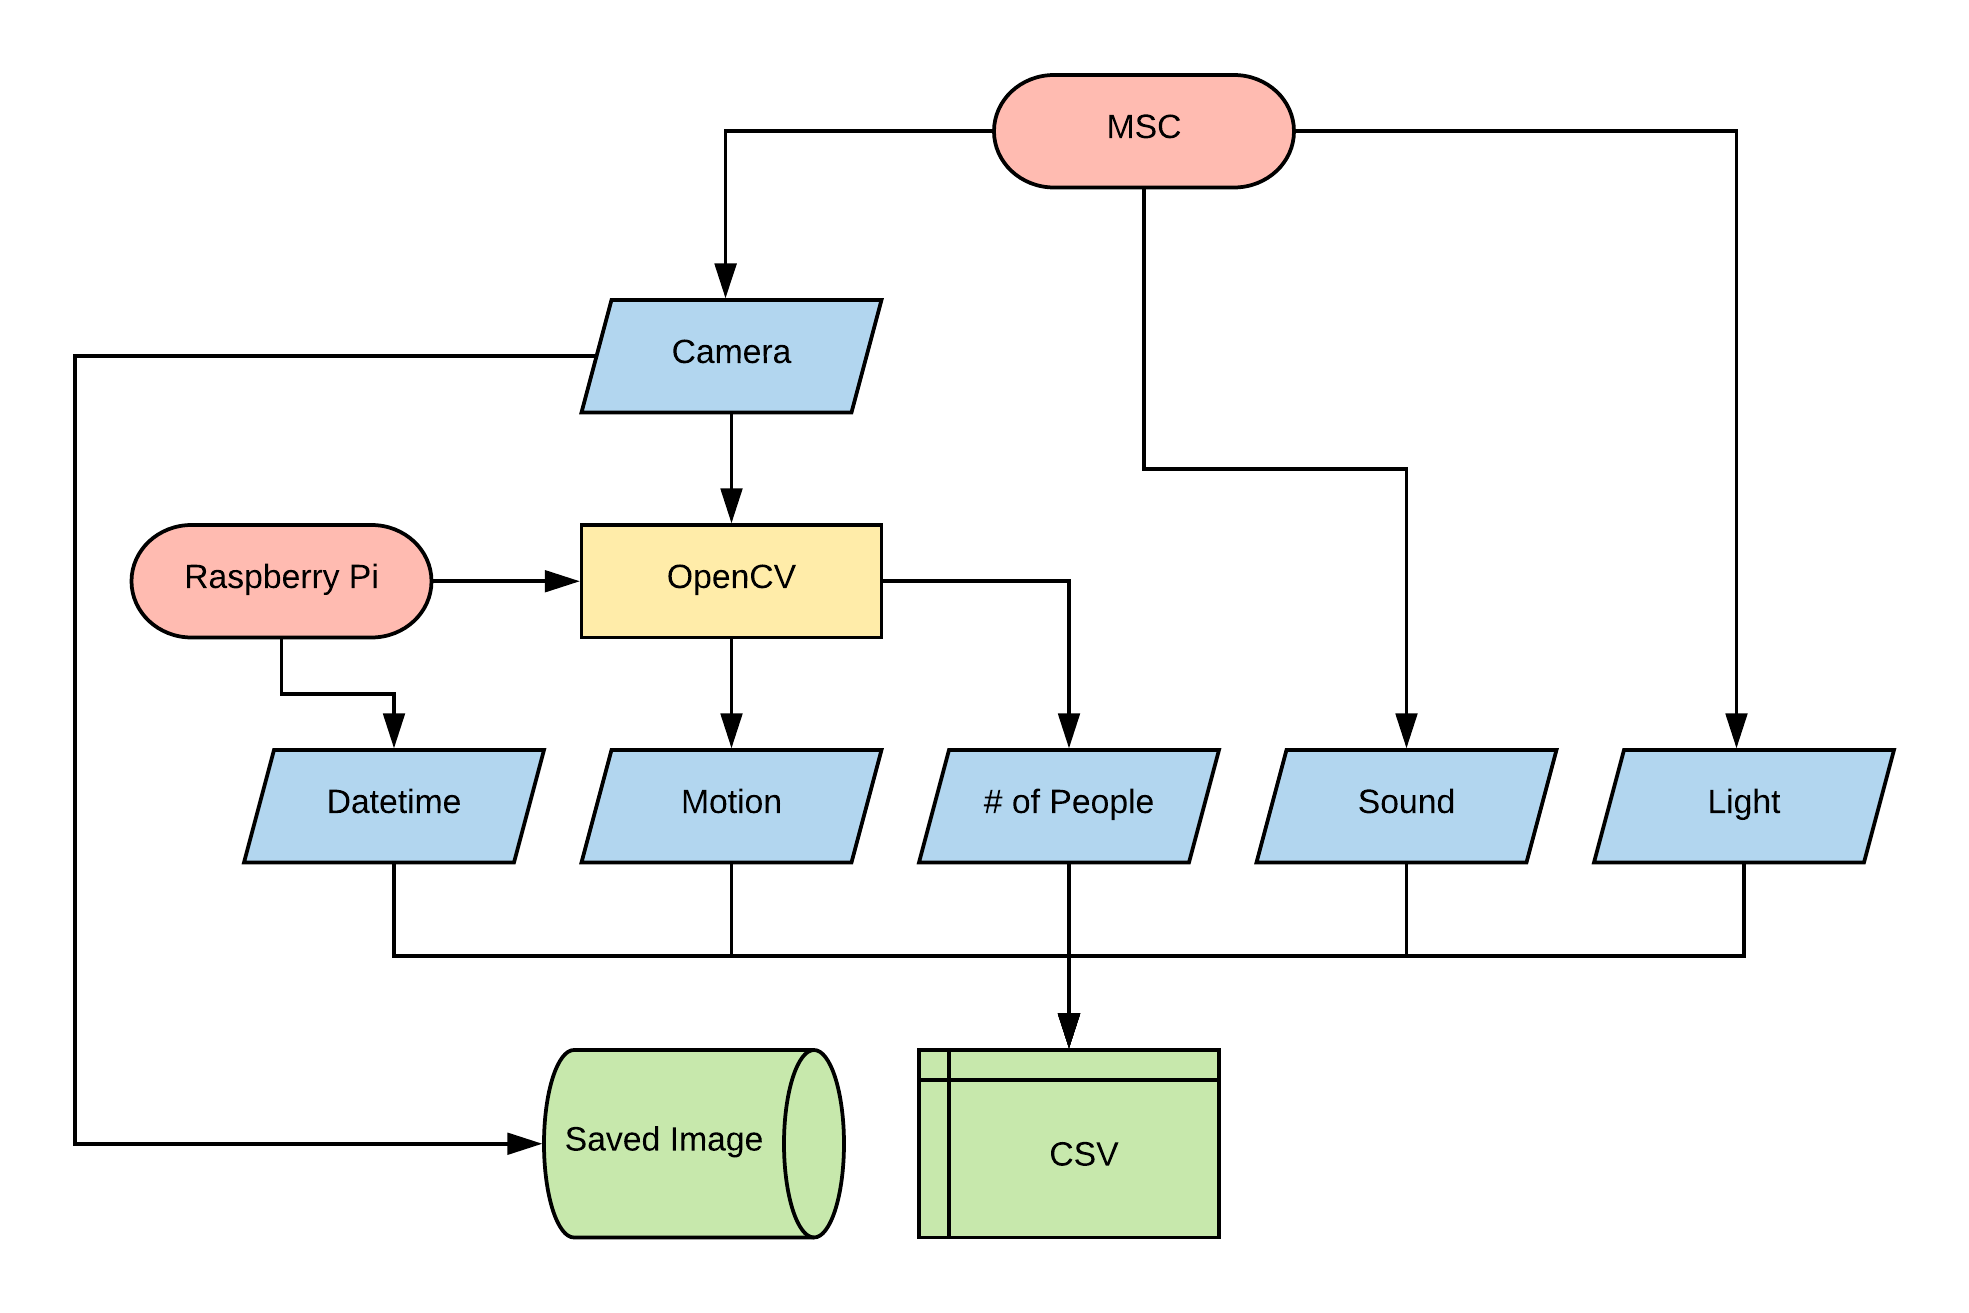
\includegraphics[width=0.97\linewidth]{figs/flowchart.png}
    \caption{Flowchart illustrating data collection and processing.}
    \label{fig:flowchart}
\end{figure}